\documentclass[conference]{IEEEtran}
\IEEEoverridecommandlockouts
% The preceding line is only needed to identify funding in the first footnote. If that is unneeded, please comment it out.
\usepackage{cite}
\usepackage{amsmath,amssymb,amsfonts}
\usepackage{algorithmic}
\usepackage{graphicx}
\usepackage{textcomp}
\usepackage{xcolor}
\usepackage{url}
\def\BibTeX{{\rm B\kern-.05em{\sc i\kern-.025em b}\kern-.08em
    T\kern-.1667em\lower.7ex\hbox{E}\kern-.125emX}}

% ==== notation macros ==== 
\newcommand{\act}{\boldsymbol{a}}          % action trajectory
\newcommand{\ind}{\mathbf{1}}              % indicator
\newcommand{\Acal}{\mathcal{A}}            % action vocabulary
\newcommand{\Mcal}{\mathcal{M}}            % compatibility relation
\newcommand{\Ccal}{\mathcal{C}}            % motion-class set
\newcommand{\todo}[1]{\textcolor{red}{[TODO: #1]}}

\begin{document}

\title{Action-Grounded VLM Reasoning for Autonomous Vehicle Semantic Anomalies\\
% {\footnotesize \textsuperscript{*}Note: Sub-titles are not captured in Xplore and should not be used}
% \thanks{Identify applicable funding agency here. If none, delete this.}
}

\author{\IEEEauthorblockN{Daniel Adejumo\textsuperscript{2}, Omkar Ankalkope\textsuperscript{2}, Kunal Runwal\textsuperscript{2}, and Aliasghar Arab\textsuperscript{1,2,$*$}}%
\thanks{\textsuperscript{1}Aliasghar Arab is with The City College of New York, Grove School of Engineering, New York, NY 10031, USA. aarab@ccny.cuny.edu}%
\thanks{\textsuperscript{2}Daniel, Omkar, Kunal and Aliasghar are with the Department of Mechanical and Aerospace Engineering, Tandon School of Engineering, New York University, 6 MetroTech Center, Brooklyn, NY 11201, USA (ASAS-Labs). aliasghar.arab@nyu.edu}%
% \thanks{\textsuperscript{$*$}Corresponding author.}%  <-- uncomment/adjust: the meaning of the asterisk was not specified
}

\maketitle

\begin{abstract}
As autonomous vehicles (AVs) scale into real-world deployment, they increasingly encounter \emph{semantic anomalies}: scenarios in which the perception stack performs exactly as designed yet the vehicle behaves incorrectly, because a familiar object appears outside its nominal context: a stop sign on a billboard, brake lights on a video screen, or a fire hose across a live lane. Vision--language models (VLMs) are increasingly adopted as a reasoning layer to close this contextual gap. However, prevailing approaches supply the VLM with scene visual data and, effectively, an ``is this anomalous?'' prompt. We show that this formulation is fundamentally ambiguous, for VLMs and arguably for humans, because a semantic anomaly scenario is defined not by the scene alone but by the ego vehicle's \emph{response} to it: the same billboard is benign if the vehicle maintains its speed and anomalous if the vehicle starts braking. Only the anomalous response grounds the anomaly and requires an external intervention. We therefore propose action-grounded anomaly reasoning, in which the VLM receives the ego vehicle's action sequence (velocity and heading over time) alongside the scene video. To support this, we introduce a systematic six-field framework for generating semantic anomalies (object, nominal context, out-of-distribution context, normal action, anomalous action, example scenario), instantiate it as a taxonomy of 112 scenario pairs spanning both failure polarities (42 grounded in documented incidents, including NHTSA recalls and NTSB investigations) and release \textbf{av\_semantic\_anomalies}, the first action-grounded semantic-anomaly dataset for AVs: world-model-generated driving videos paired with per-timestep ego-action trajectories recovered via inverse dynamics, with matched normal/anomalous clips for most scenarios. At inference, a two-stage protocol first derives the scene-required action from an action-blind early window of the clip, then checks the vehicle's actual trajectory against this expectation. Action grounding improves anomaly-classification accuracy from 74.5\% to 82.1\% (and anomaly recall from 0.54 to 0.76) over the strongest video-only baseline.
\end{abstract}

\begin{IEEEkeywords}
semantic anomaly detection, autonomous vehicles, vision--language models, action grounding, runtime monitoring, world models
\end{IEEEkeywords}

\section{Introduction}\label{sec:intro}

Autonomous vehicles (AVs) are now deployed at scale in commercial robotaxi and driver-assistance fleets, and with that scale has come a steady record of failures in which the perception stack performs exactly as designed and the vehicle nonetheless behaves incorrectly. A stop sign is correctly detected, but it is printed on a billboard. Brake lights are correctly recognized, but they belong to an advertisement on a roadside screen. A thin, flat object on the road is correctly classified as ignorable debris, but it is a charged fire hose at an active fire scene. These \emph{semantic anomalies}~\cite{b1} arise not from missed detections but from objects appearing outside their nominal context, so that the meaning of the scene, and therefore the correct driving response, diverges from what pattern recognition alone would suggest. Documented deployment incidents (robotaxis driving over deployed fire hoses, entering flooded roadways, and passing stopped school buses, several culminating in NHTSA recalls and NTSB investigations) indicate that this failure class is a persistent obstacle to safe autonomy rather than a curiosity.

Early approaches to anomaly detection in driving operated on single images. Pixel- and segmentation-level out-of-distribution (OOD) detection benchmarks such as Fishyscapes~\cite{b2} and SegmentMeIfYouCan~\cite{b3}, generative resynthesis methods~\cite{b4}, and corner-case object detection datasets such as CODA~\cite{b5} established that unknown objects can be localized in individual frames, while work on physical adversarial examples~\cite{b6} showed how easily frame-level classification is subverted. More recently, large language models and vision--language models (VLMs) have been applied to single-frame \emph{semantic} anomaly detection, using the broad world knowledge acquired in pretraining to reason about whether a scene is contextually unusual~\cite{b1}. However, a single image carries no temporal information: it cannot distinguish a plastic bag drifting across the lane from a static obstacle, a decelerating lead vehicle from a parked one, or a pedestrian about to cross from one waiting at the curb. Many semantic anomalies are defined by dynamics, and are simply not observable in a single frame.

Video-based reasoning addresses this limitation by giving the model a temporal window. Dashcam anomaly datasets such as DoTA~\cite{b7} enabled spatio-temporal detection of when and where traffic anomalies occur, language-aligned methods such as AnomalyCLIP~\cite{b8} allowed anomaly categories to be specified in natural language, and driving-tuned multimodal models (DriveGPT4~\cite{b9}, DriveVLM~\cite{b10}, and physical-AI reasoning models such as Cosmos-Reason1~\cite{b11}, further adapted by post-training frameworks such as VLM-AutoDrive~\cite{b12}) brought general-purpose reasoning to ego-video understanding. The principal objection to this line of work has been latency: multi-billion-parameter VLMs historically could not produce a verdict within the timing budget of an on-vehicle safety monitor. This speed gap, however, is closing. Recent work on a quantized semantic observer layer~\cite{b13} demonstrates that an NVFP4-quantized Cosmos-Reason1-7B with efficient attention reaches roughly 500~ms per inference, a ${\sim}50\times$ speedup over its unoptimized baseline, sufficient to run continuously at 1--2~Hz alongside the primary control loop and trigger fail-safe handoffs. Semantic video reasoning is therefore no longer blocked on deployment feasibility.

With latency fading as the binding constraint, attention shifts to the accuracy of the verdicts themselves, and here a gap persists. A single forward-facing camera view under-constrains the judgment: hazards approaching from the side, context distributed around the vehicle, and view-dependent appearance all limit what monocular video can resolve. Multi-view reasoning addresses this by exploiting the surround-view rigs standard on AV platforms~\cite{b14}. Language-enhanced bird's-eye-view representations~\cite{b15}, holistic multi-view vision-language frameworks with counterfactual reasoning~\cite{b16}, and spatio-temporal benchmarks over synchronized multi-camera video~\cite{b17} all show measurable gains from wider spatial context, and view-grounding studies~\cite{b18} confirm that models benefit when they can identify which camera holds the evidence.

Yet even with full temporal and spatial context, one crucial input remains missing: \emph{what the vehicle is doing}. We argue that this omission is not incidental but definitional. A semantic anomaly is a property of the scene--action pair, not of the scene alone. The billboard stop sign is benign if the ego vehicle drives past at speed and anomalous if the vehicle brakes for it; the fire hose scene is handled correctly if the vehicle stops and catastrophically if it proceeds. The prevailing formulation (show the model a video and ask ``is there an anomaly?'') is therefore ambiguous in principle: the same clip admits both labels depending on the ego response, an ambiguity that confronts human annotators no less than VLMs. Without the ego action, the model must guess the vehicle's behavior from subtle visual cues of ego-motion, conflating perception of the scene with inference about the response to it.

In this paper we close that gap by grounding VLM anomaly reasoning in the ego vehicle's action. Alongside the ego video, the model receives the vehicle's action sequence, velocity and heading over time, and is asked whether the \emph{behavior in context} reveals a semantic misunderstanding requiring intervention. This reframing converts an ill-posed scene-classification problem into a well-posed behavior-evaluation problem, and in our experiments it improves anomaly-classification accuracy from 74.5\% to 82.1\% (and anomaly recall from 0.54 to 0.76 at comparable specificity) over an otherwise identical video-only baseline.

A second obstacle stands in the way of this reframing: existing AV datasets cannot supervise it. Anomaly labels in current datasets (dashcam accident corpora~\cite{b7}, corner-case detection sets~\cite{b5}, and driving QA benchmarks~\cite{b16,b17}) are attached to scenes or objects, not to ego behavior, and the standard perception suites~\cite{b14} contain almost no semantic-anomaly content at all. Scene-level labels inherit exactly the ambiguity described above: a clip labeled ``anomalous'' does not specify whether the anomaly lies in the world or in the vehicle's response to it. What is needed is a dataset in which each scenario appears with \emph{both} polarities of ego behavior, a correct response and an incorrect one, each paired with the corresponding action trajectory, so that the label is unambiguous by construction.

We construct such a dataset. Building on a systematic six-field framework for generating semantic anomalies (object, nominal context, OOD context, normal action, anomalous action, and example scenario), we develop a taxonomy of 112 scenario pairs spanning both failure polarities (acting on a non-threat and failing to act on a disguised threat), 42 of them grounded in documented real-world incidents including NHTSA recalls, NTSB investigations, and published adversarial-ML attacks. From this taxonomy we release \textbf{av\_semantic\_anomalies}, to our knowledge the first action-grounded semantic-anomaly dataset for AVs: world-model-generated ego-view driving videos in matched normal/anomalous pairs, each accompanied by a per-timestep ego-action trajectory (velocity and heading at 5~Hz and 10~Hz) recovered via inverse dynamics and validated both heuristically and manually.

The contributions of this paper are threefold. First, we identify and formalize the action-grounding gap in VLM-based semantic anomaly detection, showing that scene-only inference is inherently ambiguous because the anomaly label is defined by the scene--action pair. Second, we propose action-grounded anomaly reasoning, in which the VLM receives the ego action sequence alongside video, and demonstrate an improvement in classification accuracy from 74.5\% to 82.1\%, with anomaly recall rising from 0.54 to 0.76. Third, we release the six-field generation framework, the 112-pair incident-grounded taxonomy, and the av\_semantic\_anomalies dataset to enable training and evaluation of action-aware anomaly detectors.

The remainder of this paper is organized as follows. Section~\ref{sec:method} presents the methodology: the semantic-anomaly definition framework, synthetic video generation, action extraction from the synthetic video data, and the VLM context and anomaly-reasoning approach. Section~\ref{sec:results} reports results: the released dataset, the VLM performance evaluation, and ablations. Section~\ref{sec:conclusion} concludes.

\section{Methodology}\label{sec:method}

\subsection{Semantic Anomalies Definition Framework}\label{sec:framework}

We define a \emph{semantic anomaly} as a driving failure in which the perception stack performs as designed (the object is detected, and often correctly classified), yet the vehicle behaves incorrectly because the object appears outside its nominal context and the system misreads what the scene means~\cite{b1}. The detector sees a stop sign and it \emph{is} a stop sign; the failure is that the sign is printed on a billboard rather than mounted at an intersection, so that the mandated response no longer applies. Semantic anomalies are thus disjoint from the pixel-level unknowns targeted by OOD segmentation benchmarks~\cite{b2,b3}: the object is in-distribution, but its \emph{context} is not. In the vocabulary of ISO 21448 (SOTIF), they occupy the space of scenarios that are unsafe despite the absence of any component fault~\cite{b19}.

To create a structured way of defining anomalous scenarios where semantics is the failure point, we draw on the tradition of systematic hazard enumeration in safety engineering. Hazard analysis and risk assessment (HARA) under ISO 26262~\cite{b20} decomposes vehicle functions into hazardous events via guided decomposition, and scenario-based testing similarly factors driving scenarios into functional, logical, and concrete layers~\cite{b21}. Recent work automates these analyses with generative AI, showing that LLMs can enumerate hazardous scenarios at a coverage and consistency that manual expert analysis struggles to match~\cite{b22}, an approach now productized in AI safety-engineering platforms such as General Autonomy's G-Assess~\cite{b23}. These methods, however, enumerate hazards top-down from vehicle \emph{functions} (e.g., unintended acceleration) and remain agnostic to the perceptual mechanism of failure. Our framework instead factors the anomaly bottom-up around a \emph{driving entity and its context}, and, critically, defines the anomaly label not by the scene but by the ego vehicle's action within it, consistent with the action-grounding argument of Section~\ref{sec:intro}.

Concretely, every scenario is decomposed into the six fields of Table~\ref{tab:framework}, where each field's output is the next field's input. Fields 1--3 build the scene: a semantically loaded object with a mandatory behavioral response is selected, its nominal context, where reacting to it is correct, is pinned down, and the object (or a visual look-alike) is then displaced into an out-of-distribution (OOD) context while its appearance is preserved. The displacement is performed by a small set of reusable operators: \emph{relocate} (fire hose moved into the roadway), \emph{reprint} (stop sign on a billboard or t-shirt), \emph{carry as cargo} (deactivated traffic signals on a flatbed), \emph{reflect} (signage in a mirrored facade), \emph{project} (a phantom pedestrian projected on the pavement), and \emph{natural mimic} (a low moon resembling a signal lamp). Fields 4--5 define the behavioral contrast in that OOD context: the Normal Action of a context-aware driver, who responds to the scene rather than the pattern, and the Anomalous Action of a purely pattern-matching stack, which responds to the pattern as if it were in its nominal context. Field 6 collapses the row into a one-sentence concrete scenario, directly usable as a video-generation or evaluation prompt seed.

\begin{table}[htbp]
\caption{The six-field semantic-anomaly framework}
\begin{center}
\small
\begin{tabular}{|c|l|p{4.6cm}|}
\hline
\textbf{\#} & \textbf{Field} & \textbf{Description} \\
\hline
1 & Object in Driving Scene & Semantically loaded entity with a mandated response (stop sign, brake lights, pedestrian, fire hose) \\
\hline
2 & Nominal Context & Where the object normally lives and where reacting to it is correct \\
\hline
3 & OOD Context & Displacement of the object or a look-alike outside its nominal context, appearance preserved (relocate, reprint, carry as cargo, reflect, project, natural mimic) \\
\hline
4 & Normal Action in OOD & What a context-aware driver correctly does: respond to the scene, not the pattern \\
\hline
5 & Anomalous Action in OOD & The failure mode: respond to the pattern as if in its nominal context, or fail to respond to a real hazard presenting atypically \\
\hline
6 & Example Scenario & One-sentence concrete description; the video-generation / evaluation prompt seed \\
\hline
\end{tabular}
\label{tab:framework}
\end{center}
\end{table}

Because fields 4 and 5 attach \emph{both} a correct and an incorrect ego behavior to the same scene, every row of the framework yields a \emph{scenario pair}: two clips of an identical situation that differ only in the ego vehicle's action, one labeled Normal and one labeled Anomalous. This pairing is what makes the anomaly label unambiguous by construction (the label is a property of the scene--action pair), and it covers both failure polarities. In a \emph{false-positive} (FP) failure the vehicle acts on a non-threat: braking for the billboard sign, phantom-braking for an overpass shadow. In a \emph{false-negative} (FN) failure the vehicle ignores a disguised real threat: driving over a charged fire hose, entering a flooded road that reads as wet pavement. Both polarities share the same root cause, pattern recognition without contextual reasoning, and Table~\ref{tab:examples} shows one instantiated row of each.

\begin{table*}[htbp]
\caption{Example scenario pairs, one per failure polarity}
\begin{center}
\small
\begin{tabular}{|p{1.4cm}|p{2.4cm}|p{2.7cm}|p{2.6cm}|p{2.5cm}|p{3.2cm}|c|}
\hline
\textbf{Object} & \textbf{Nominal Context} & \textbf{OOD Context} & \textbf{Normal Action} & \textbf{Anomalous Action} & \textbf{Example} & \textbf{Tag} \\
\hline
Fire hose & Coiled on a fire engine, off the roadway & Charged hose laid across an active lane at a fire scene & Stop before the hose; never cross; wait to be waved through & Classifies it as debris and drives over the hose & A car drives over a charged fire hose stretched across the street at an active fire scene & REAL $\cdot$ FN \\
\hline
Brake lights & Rear of a lead vehicle in the ego lane & Life-size car ad with glowing brake lamps on a night digital billboard & Recognize the screen as media; hold speed and lane & Reads a braking lead vehicle and brake-checks at speed & A car brake-checks for brake lights shown on a nighttime video billboard & SYN $\cdot$ FP \\
\hline
\end{tabular}
\label{tab:examples}
\end{center}
\end{table*}

The framework is anchored in deployment reality. Each row carries a provenance tag: \textbf{REAL} rows are derived from documented incidents, NHTSA recalls, NTSB investigations, peer-reviewed adversarial-ML attacks, and verified incident reporting. The fire-hose row of Table~\ref{tab:examples} reproduces documented Cruise incidents at San Francisco fire scenes (2022--2023), where robotaxis drove over deployed hoses until firefighters physically intervened~\cite{b24}; other REAL rows include a Tesla on Autopilot repeatedly stopping for a Burger King logo it read as a stop sign~\cite{b25}, a taped ``35'' speed sign read as ``85'' that accelerated a Tesla's cruise control~\cite{b26}, a Waymo that entered a flooded San Antonio roadway and was swept into a creek, triggering a 3{,}791-vehicle recall~\cite{b27}, and a Waymo that passed a stopped school bus after a remote operator misjudged its signals, prompting an NTSB investigation~\cite{b28}. Grounding the taxonomy in incidents that produced recalls and federal investigations ensures that the dataset targets failure modes with demonstrated, not hypothetical, safety impact.

\textbf{SYNTHETIC} rows are then generated by applying the same pattern to new object--context combinations: hold the framework logic fixed (same object class discipline, a displacement operator from the standard set, a correct action, and a plausible pattern-matching failure) and extrapolate. The brake-lights row of Table~\ref{tab:examples} is one such extrapolation: no specific incident is on record, but its mechanism class is documented, phantom responses to split-second signs injected into digital billboards~\cite{b29}, making the synthetic row a valid, incident-adjacent hypothesis rather than an invention. Worked in tabular form, the framework also supports parallel authoring (one object row spawns many OOD-context rows), completeness checking (an empty cell is a visible gap), and polarity balancing (FP/FN tags are countable). Applied this way, the framework produced a 12-row seed taxonomy and a 100-row extension for a total of 112 scenario pairs across ten categories, of which 42 are REAL and 70 are SYNTHETIC. \todo{REAL/SYNTHETIC tags for 12 rows pending; the count of 70 is tentative.} The ten categories are traffic-control-device look-alikes; pedestrian and humanoid confusions; animal anomalies; weather, smoke, and lighting; road surface and markings; unusual cargo and vehicles; emergency and event scenarios; adversarial and projected attacks; reflections and screens; and infrastructure, rail, and operational anomalies. Each row's Example field seeds the synthetic video generation described in Section~\ref{sec:videogen}, and each Normal/Anomalous pair supplies the binary behavior labels used throughout the rest of the paper.

\subsection{Synthetic Video Generation}\label{sec:videogen}

Semantic anomalies are, by construction, rare: the scenarios of Section~\ref{sec:framework} appear in deployment logs only as isolated incidents, and several (the synthetic rows) have not yet been observed at all. Collecting a balanced corpus of real footage (much less footage of the \emph{anomalous} ego behavior, which no operator would deliberately produce) is therefore impractical. We instead synthesize the dataset with the Cosmos~3 world foundation model~\cite{b30}, generating a paired ego-view video for each polarity of every scenario. Each row's Example field (framework field 6) serves as the generation seed, extended with the Normal or Anomalous action of fields 4--5, so that the two clips of a pair depict the same scene and differ only in the ego vehicle's behavior. The pipeline comprises five stages: prompt upsampling, human validation of the dense prompts, scenery variation, video generation, and human validation of the generated videos.

\paragraph{Prompt upsampling} The framework's one-sentence scenario seeds are deliberately sparse, concise enough to author and audit at taxonomy scale, but text-to-video generation benefits from dense, unambiguous scene specifications. Each sparse prompt is therefore expanded by an LLM-based prompt upsampler into a structured Cosmos~3 JSON prompt specifying the subjects (with counts), background setting, lighting, cinematography, on-screen text and signage, and a segmented action timeline with per-segment temporal captions. The upsampler preserves the scenario's semantic core (the object, its OOD context, and the ego action) while filling in the photometric and geometric detail the sparse seed leaves open.

\paragraph{Anomaly-defining action timing} Because the Normal/Anomalous label is carried by the ego action rather than the scene, the clip must devote sufficient duration to the label-defining behavior. Each prompt's action timeline is authored so that the final segment, which contains the correct response or the failure (e.g., the full stop before the fire hose, or the vehicle rolling over it), spans at least 2~s of the clip, and deceleration profiles are constrained to physically plausible windows (a smooth stop from cruising speed occupies roughly 2.5--4~s rather than an instantaneous halt). This guarantees that the behavioral contrast between the two clips of a pair is temporally resolvable, both by the downstream inverse-dynamics action recovery of Section~\ref{sec:action} and by the VLM at inference time.

\paragraph{Human validation of dense prompts} Upsampled prompts undergo a two-round human-in-the-loop realism review. In the first round, each dense prompt is audited field-by-field against a realism rubric covering lighting and shadow consistency, motion physics, geometry and perspective, traffic-infrastructure norms, object counts and legibility, and internal cross-field contradictions; the \emph{intended} anomaly is explicitly exempt (it is the point of the scenario, not a defect) and must survive every edit. Identified implausibilities are corrected in the sparse source prompt, which is then re-upsampled. In the second round, any residual implausibilities are fixed directly in the regenerated JSON, and every change is logged to an auditable review report. This separates the two failure modes of synthetic data: the review removes \emph{unintended} distribution shift (physically impossible lighting, implausible braking) while preserving the \emph{intended} semantic shift that defines the anomaly.

\paragraph{Scenery variation} Each validated dense prompt is then expanded into a family of roughly twenty scenery variations, varying weather, lighting, time of day, and urban context while preserving the scenario's semantic core (the object, its OOD context, and the ego action), so that each scenario polarity is represented by a visually diverse clip family rather than a single rendering.

\paragraph{Video generation} Validated prompts are rendered by the Cosmos~3 text-to-video model, served through a vLLM Omni inference stack. Each prompt yields a 5-second (in a minority of scenes, 8-second), $832\times480$, 24~fps ego-view clip. Generation was performed with the Cosmos3-Nano variant on a single GPU, with the larger Cosmos3-Super variant supported on a 4-GPU tensor-parallel configuration for higher-fidelity replication.

\paragraph{Human validation of generated videos} Finally, each generated clip is reviewed by a human against its sparse source scenario: the reviewer confirms that the intended object, OOD context, and, critically, the intended ego action are all depicted, and flags residual generation artifacts or scenario drift. Feedback at this stage is folded back into the sparse prompts and the affected clips are regenerated, closing the loop between scenario authoring and video synthesis. Clips that pass review constitute the paired Normal/Anomalous videos of the dataset.

Applied to the 12-row seed taxonomy of Section~\ref{sec:framework}, this pipeline produces the current video corpus of the \textbf{av\_semantic\_anomalies} dataset, released openly on Hugging Face.\footnote{\url{https://huggingface.co/datasets/ASASLab/av_semantic_anomalies}} Section~\ref{sec:action} describes how ego-action trajectories are recovered from these clips, and Section~\ref{sec:dataset} details the resulting dataset structure.

\subsection{Action Extraction from Synthetic Video Data}\label{sec:action}

Text-to-video generation produces pixels, not telemetry: the clips of Section~\ref{sec:videogen} depict an ego action but do not come with the action signal itself. To ground VLM reasoning in what the vehicle is doing, we recover each clip's ego-action trajectory using the Cosmos~3 video-to-action inverse-dynamics pipeline, executed with the Cosmos3-Nano model.

Each 24~fps clip is first temporally resampled to 10~fps (7.5~fps for the 8~s clips) so that the inverse-dynamics model's fixed 61-frame input window spans the entire clip rather than a 2.5~s prefix. The model then predicts a frame-to-frame ego-motion trajectory, per-step translation and rotation (a 9-dimensional translation + 6D-rotation parameterization over the $T-1$ frame transitions). The relative poses are composed into absolute camera-to-world poses and scaled to metric units, from which we derive the two action channels used throughout this work: ego \textbf{velocity} (mph) and ego \textbf{heading} (degrees, relative to the first frame). Each clip thus yields a time-stamped action sequence of [velocity, heading] pairs at the resampled native rate (10~Hz; 7.5~Hz for the 8~s clips), together with a 5~Hz downsampled variant for token-budget-constrained VLM contexts. These two channels are deliberately chosen to mirror a real vehicle's most basic proprioceptive sensors, wheel-speed odometry and steering/yaw measurement, so that a reasoning model trained or evaluated on the synthetic action format transfers directly to the velocity and steering-angle signals available on any production CAN bus, without requiring privileged simulator state.

Recovered trajectories are validated in two stages. First, an automated heuristic check compares the tail of each trajectory against the final action sentence of its source prompt, the label-defining segment of Section~\ref{sec:videogen}: a clip whose prompt ends in a full stop before the fire hose should terminate near zero velocity, while its anomalous twin should not. Trajectories violating these expectations are flagged for inspection. Second, every trajectory undergoes manual validation in a purpose-built review interface that plays each video alongside its synchronized velocity and heading plots; a human reviewer judges whether the recovered action is \emph{realistic} (physically plausible magnitudes and smoothness) and \emph{faithful} (consistent with the motion visible in the clip), and records a Valid/Invalid label with free-text comments alongside the heuristic verdict. Clips whose trajectories fail validation are regenerated or excluded. Regeneration is closed-loop and acceptance-gated: the source prompt is re-rendered under multiple seeds, and a candidate clip is accepted only when two automated witnesses, the recovered inverse-dynamics trajectory and an independent optical-flow motion probe, agree with the prompted ego action; 68 clips of the current release entered through this gate, and scenarios for which no candidate passed were excluded. Every action sequence in the released dataset therefore carries both automated and human plausibility checks.

The output of this stage (paired Normal/Anomalous clips, each with validated 5~Hz and 10~Hz [velocity, heading] trajectories) is the action grounding that Section~\ref{sec:vlm} supplies to the VLM; the packaging of the released dataset is described in Section~\ref{sec:dataset}.

\subsection{VLM Context and Anomaly Reasoning}\label{sec:vlm}

\begin{figure*}[!t]
\centering
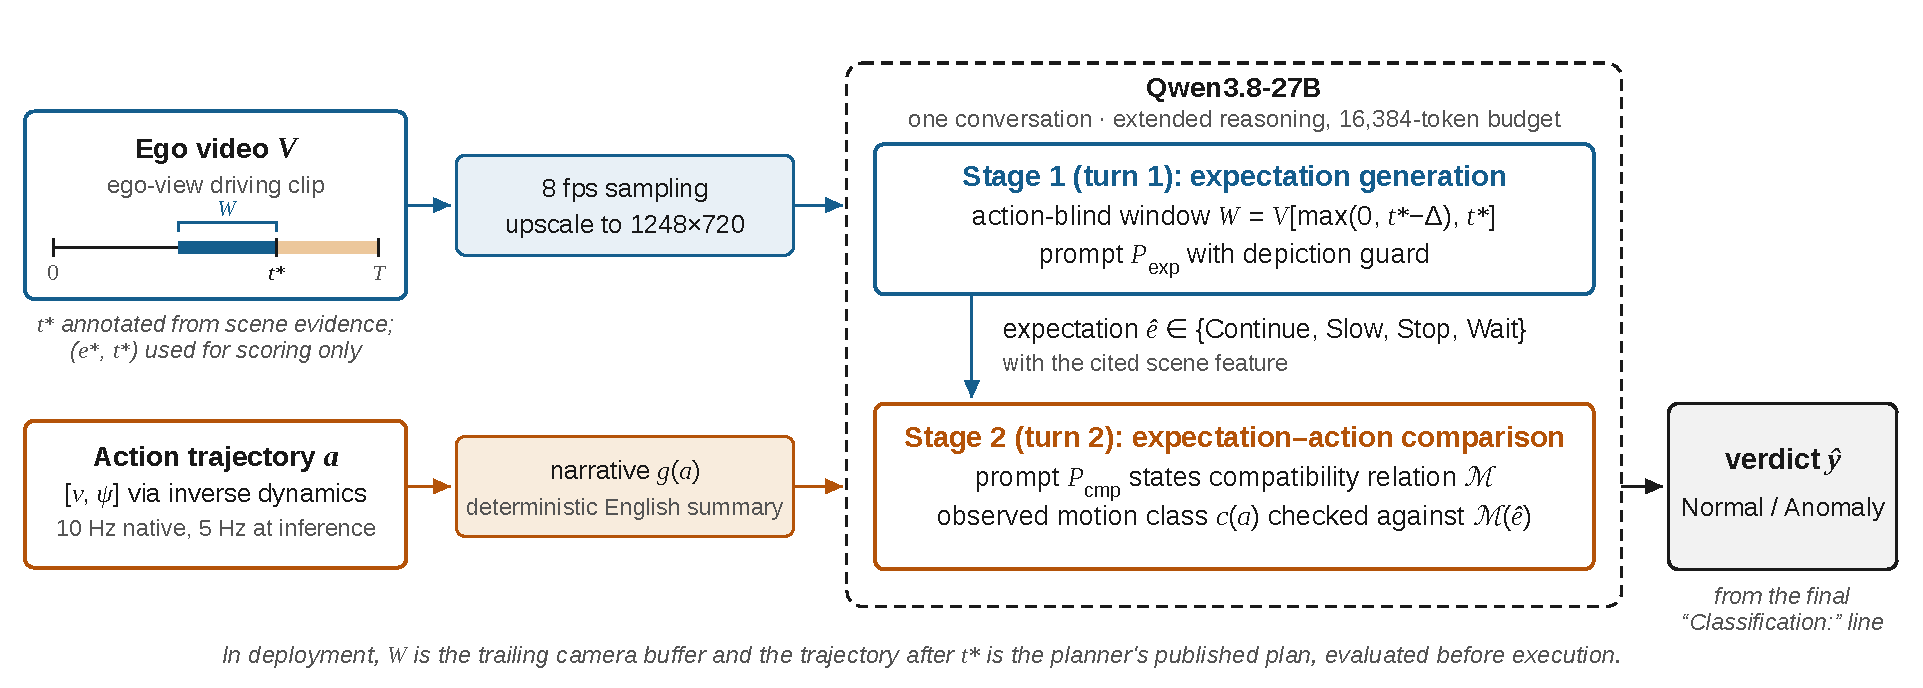
\includegraphics[width=\textwidth]{fig_pipeline_color.pdf}
\caption{The two-stage expectation--action anomaly monitor (video path in blue, action path in orange). Stage 1 sees only the action-blind window $W$ ending at the clip's decision time $t^*$ and produces the expected action $\hat{e}$; stage 2 compares the deterministic narrative rendering $g(\act)$ of the actual trajectory against the compatibility relation $\Mcal(\hat{e})$, yielding the verdict $\hat{y}$ of~\eqref{eq:label}.}
\label{fig:pipeline}
\end{figure*}

\paragraph{Problem formulation} Let $V = (x_1, \dots, x_N)$ denote an ego-view clip of duration $T$ and let $\act = ((v_1, \psi_1), \dots, (v_K, \psi_K))$ be its recovered action trajectory (Section~\ref{sec:action}), sampled at $f = 5$~Hz so that $K = fT$. The prevailing scene-only formulation trains or prompts a classifier $h(V) \rightarrow \{\text{Normal}, \text{Anomaly}\}$; as argued in Section~\ref{sec:intro}, this map is ill-posed because the label is a property of the scene--action pair. We therefore factor the judgment. Let $\Acal = \{\text{Continue}, \text{Slow}, \text{Stop}, \text{Wait}\}$ be a coarse action vocabulary, let $e^* \in \Acal$ be the action a correct, context-aware driver should take in the depicted scene (framework field 4, Section~\ref{sec:framework}), and let $c(\act)$ be the motion class actually realized by the trajectory, drawn from the observable set $\Ccal = \{\text{continued}, \text{slowed}, \text{stopped}, \text{waited}, \text{moved off}\}$. The anomaly label is then, by construction,
\begin{equation}
y = \ind\!\left[\, c(\act) \notin \Mcal(e^*) \,\right],\label{eq:label}
\end{equation}
where $\Mcal : \Acal \rightarrow 2^{\Ccal}$ is a fixed compatibility relation (defined below) that maps each expected action to the motion classes that satisfy it. Equation~\eqref{eq:label} decomposes anomaly detection into two strictly simpler subproblems: \emph{expectation generation}, inferring $e^*$ from the scene alone, and \emph{expectation--action comparison}, testing membership in $\Mcal(e^*)$. Our inference protocol instantiates each subproblem as one turn of a single VLM conversation (Fig.~\ref{fig:pipeline}), an arrangement in the spirit of model-predictive runtime monitors that flag divergence between what should happen and what does happen~\cite{b31}, but with the ``should'' produced zero-shot by the VLM's world knowledge rather than by a learned dynamics model.

\paragraph{Model and serving} Both stages are executed zero-shot by Qwen3.8-27B~\cite{b32}, an open-weight vision--language model with native video input and extended (chain-of-thought) reasoning~\cite{b33}, selected over the driving-tuned alternative of~\cite{b11} and five other open VLMs in the model comparison of Section~\ref{sec:ablations}. The model is served through vLLM~\cite{b34} with its reasoning parser enabled, a 32{,}768-token context, and a fixed seed; the identical decoding configuration is used for both stages: the model card's reasoning settings (temperature 1.0, top-$p$ 0.95, top-$k$ 20) with a 16{,}384-token generation budget.

\paragraph{Input preprocessing} Video is sampled at 8~fps and upscaled from the native $832\times480$ to $1248\times720$ (Lanczos) before encoding. Upscaling adds no scene information; its effect is architectural. The vision encoder allocates visual tokens by pixel area, so the same frame spans $2.25\times$ more pixels at 720p (in practice ${\approx}\,1.5\times$ more visual tokens under the processor's total-pixel budget), and small discriminative details (a printed sign, a deflated balloon at range) that fall below one patch at 480p survive patchification at the higher resolution. This single preprocessing change is among the largest accuracy levers we found (Section~\ref{sec:ablations}); a 2.5~s window encodes to ${\approx}\,8.8$k visual tokens. The context uses the single forward ego view, matching the single-view synthetic corpus; the multi-view extensions of~\cite{b15,b16,b17,b18} are orthogonal and complementary.

\paragraph{Stage 1: expectation from an action-blind window} The first turn supplies only an early video window
\begin{equation}
W = V\big[\max(0,\; t^* - \Delta),\; t^*\big], \qquad \Delta = 2.5~\mathrm{s},\label{eq:window}
\end{equation}
together with the expectation prompt $P_{\mathrm{exp}}$ of Fig.~\ref{fig:prompts}, and elicits $\hat{e} = f_\theta(W, P_{\mathrm{exp}}) \in \Acal$: what a correct driver \emph{should} do over the next few seconds, plus the specific real scene feature that requires it. Two design choices carry the weight here. First, the window ends at the clip's \emph{decision time} $t^*$, the earliest instant at which the correct action is determinable from the scene, which defaults to $T - 2.5$~s and is annotated per clip (from scene evidence only, never from the ego motion) where the hazard develops later; the ground-truth pair $(e^*, t^*)$ extends the taxonomy labels of Section~\ref{sec:framework} and is used exclusively for scoring, never in any prompt. Ending the window at $t^*$ keeps stage 1 blind to the label-defining behavior: when we instead exposed the full clip, the ``expectation'' anchored on the visible ego action (a braking vehicle induces the expectation \emph{Stop}, which then trivially matches), collapsing exactly into the ambiguity of~\eqref{eq:label} that action grounding is meant to remove. Second, $P_{\mathrm{exp}}$ embeds a \emph{depiction guard}: an apparent traffic control or hazard that is only an image (printed, painted, displayed, reflected, worn, or carried) commands nothing. This single sentence supplies the contextual rule that defines the semantic-anomaly class, a rule that prompt-only scene classification consistently misapplies (Section~\ref{sec:ablations}).

\paragraph{Stage 2: comparison against the actual action} The second turn of the same conversation supplies the actual trajectory $\act$ over the full clip and the comparison prompt $P_{\mathrm{cmp}}$ of Fig.~\ref{fig:prompts}. Rather than the raw number sequence, the trajectory is rendered by a deterministic \emph{mechanical narrative} $g(\act)$: with $\bar{v}_0$ the mean of the first three speed samples and $\bar{v}_1$ the mean of the last three, the renderer emits exactly one clause: \emph{moved off} ($\bar{v}_0 \leq 2$~mph $\wedge$ $\bar{v}_1 \geq 5$~mph), \emph{stopped} ($v_K \leq 2$~mph $\wedge$ $\bar{v}_0 > 5$~mph), \emph{slowed} ($\bar{v}_1 \leq 0.6\,\bar{v}_0$), \emph{sped up} ($\bar{v}_1 \geq 1.4\,\bar{v}_0$), else \emph{held steady}, with the quantities inlined (``the vehicle slowed from about 21 mph to a complete stop and was stationary at the end''), appending a heading clause when $\max_k |\psi_k| \geq 10^{\circ}$. Because $g$ is pure arithmetic over the same numbers, it can leak no information beyond the trajectory itself; what it removes is the numeric-reading step, a known failure surface of LLMs over serialized time series~\cite{b35,b36}. The effect is large: given a correct stage-1 expectation, the comparator is essentially perfect with the narrative rendering but errs on 17--30\% of clips when handed the raw $[[v, \psi], \dots]$ list (Section~\ref{sec:ablations}). $P_{\mathrm{cmp}}$ also states $\Mcal$ explicitly rather than leaving compatibility implicit: \emph{continue} and \emph{slow} are mutually compatible (a mild slowdown is not an intervention-worthy mismatch), an expected \emph{stop} is satisfied by coming to rest or remaining at rest, and the residual combinations (stopping when continue/slow was expected, failing to stop when stop was expected, moving off when wait was expected) are mismatches. The model states the observed motion class, compares, and emits the verdict $\hat{y}$ on its final line.

\paragraph{Reasoning mode} Both stages run with extended reasoning enabled: the model produces a delimited reasoning trace before its answer~\cite{b33,b37}. This is not incidental: with reasoning disabled (direct response, card-recommended non-reasoning sampling), the same prompts lose 8--12 accuracy points (Section~\ref{sec:ablations}), with the loss concentrated in the depiction-trap scenarios where the correct verdict requires explicitly weighing the guard rule against the visual pattern. Generation that exhausts the reasoning budget is \emph{not} resampled or extended; it is scored as described next.

\paragraph{Output parsing} The serving stack's reasoning parser separates the trace from the answer body, and only the answer can produce a decision. The stage-1 answer is the option word leading the final non-empty line; the stage-2 verdict is the \emph{last} ``Classification:'' match in the answer body. There is deliberately no keyword-frequency fallback: reasoning traces rehearse both labels, and scanning them resolves nearly every malformed output to Anomaly. An output with no parseable decision, including budget-truncated generations, is recorded as Unknown and scored as incorrect, so parsing failures can only hurt, never inflate, the reported numbers. All raw outputs are retained, making every verdict re-derivable offline. (In the final configuration this path is exercised rarely: zero truncations and $<1\%$ Unknown across the evaluation of Section~\ref{sec:eval}.)

\begin{figure*}[htbp]
\centering
\fbox{\begin{minipage}{\dimexpr\textwidth-2\fboxsep-2\fboxrule\relax}\small
\textbf{System prompt:} ``You are a helpful assistant.''

\medskip
\textbf{Stage 1 ($P_{\mathrm{exp}}$), with the early window $W$ attached:} ``You are evaluating the driving scene in this clip from the ego vehicle's point of view. Based only on what the scene requires---not on how the ego vehicle happens to be moving---what SHOULD a correct, safe driver do over the next few seconds? Name the specific real feature of the scene that requires it, or state that nothing requires a change. Note: an apparent traffic control or hazard that is only an image---printed, painted, displayed on a screen, reflected, worn on clothing, or carried as cargo---commands nothing. Then reply on the final line with exactly one word: Continue, Slow, Stop, or Wait. [the four options, each with a one-line gloss]''

\medskip
\textbf{Stage 2 ($P_{\mathrm{cmp}}$), second turn of the same conversation:} ``Measured from the ego vehicle's own motion sensors over the recorded $\{T\}$ seconds of this clip: $\{g(\act)\}$. Read that motion as exactly one of: continued (speed roughly held), slowed (speed clearly reduced but still moving at the end), stopped (came to rest and stayed there), waited (stationary throughout), or moved off (pulled away from a standstill). Compare it with the expectation you gave. The behaviour MATCHES the expectation only for the action that was expected, with two tolerances: `continue' and `slow' are compatible with each other, and an expected `stop' is satisfied by coming to rest or remaining at rest. Stopping when continue or slow was expected, continuing or merely slowing when stop was expected, and moving off when wait was expected are mismatches. First state the observed motion class in one short sentence. Then reply on the final line with exactly one of: Classification: Anomaly---the behaviour does not match the expected action / Classification: Normal---the behaviour matches the expected action.''
\end{minipage}}
\caption{The two prompts of the expectation--action protocol, verbatim.}
\label{fig:prompts}
\end{figure*}

\paragraph{Deployment correspondence} The two-stage protocol is constructed to map directly onto a runtime monitor. On a vehicle at wall-clock time $t$, stage 1's window is the trailing camera buffer $V[t - 2.5,\, t]$, a rolling 2.5~s window re-evaluated continuously, so the per-clip decision time $t^*$ of~\eqref{eq:window} is simply the step at which the rolling monitor first has sufficient evidence, and annotating it makes the offline evaluation measure the same quantity a continuous monitor would realize. Stage 2's trajectory decomposes at $t^*$: the segment before $t^*$ is the vehicle's recorded trajectory history, velocity and heading profiles from the same proprioceptive channels our synthetic trajectories mirror (Section~\ref{sec:action}), while the segment after $t^*$ corresponds not to a recorded outcome but to the \emph{planned} trajectory published by the vehicle's autopilot stack for the next ${\approx}\,2.5$~s. The deployed monitor therefore feeds stage 2 the concatenation of recorded history and planned horizon; our offline evaluation supplies exactly this object, with the clip's realized post-$t^*$ motion standing in for the plan. Comparing the scene-derived expectation against the planner's intent means a mismatch (the plan brakes for a printed sign, or fails to brake for a charged hose) is flagged \emph{before the action is executed}, in time to gate the plan or trigger a fail-safe handoff~\cite{b13,b31}. Nothing in the context (a camera window, two proprioceptive channels, and two fixed prompts) requires privileged simulator state.

\section{Results}\label{sec:results}

\subsection{Dataset}\label{sec:dataset}

The primary artifact of the pipeline of Section~\ref{sec:method} is the \textbf{av\_semantic\_anomalies} dataset, released openly on Hugging Face. The taxonomy of Section~\ref{sec:framework} (112 scenario pairs spanning ten categories, both failure polarities, and REAL/SYNTHETIC provenance, 42/70) seeds the corpus. The current release instantiates its 12-row seed taxonomy as scenery-varied clip families (Section~\ref{sec:videogen}); most scenario families are represented in both polarities, each Normal/Anomalous pair depicting the same scene under the correct and the incorrect ego action, so that the anomaly label is carried entirely by the vehicle's behavior. \todo{instantiate the 100-row extension before publication and update the corpus figures.}

Each video is a 24~fps ego-view clip at $832\times480$ (480p), 5~s long (21 clips: 8~s), generated with Cosmos3-Nano (Section~\ref{sec:videogen}) and released together with its recovered ego-action trajectory (Section~\ref{sec:action}). Every clip carries two action files: the native-rate sequence at 10~Hz (7.5~Hz for the 21 8-second clips, Section~\ref{sec:action}) and a downsampled variant at 5~Hz, each a time-ordered list of [velocity (mph), heading (deg)] pairs with heading expressed relative to the clip's first frame. The two rates serve different consumers: the 10~Hz sequence preserves the full temporal resolution of the inverse-dynamics model for analysis and training, while the 5~Hz variant halves the token footprint for context-window-constrained VLM inference; both carry the automated and manual validation of Section~\ref{sec:action}. In total the release comprises 315 videos with 630 trajectory files (two rates per clip), totaling 1.09~GB; Table~\ref{tab:dataset} summarizes the release.

\begin{table}[htbp]
\caption{av\_semantic\_anomalies at a glance}
\begin{center}
\small
\begin{tabular}{|l|p{4.6cm}|}
\hline
\textbf{Property} & \textbf{Value} \\
\hline
Scenario pairs (taxonomy) & 112 (42 REAL / 70 SYNTHETIC; both failure polarities) \\
\hline
Video clips & 315, in matched Normal/Anomalous pairs \\
\hline
Clip format & 5~s (21 clips: 8~s), $832\times480$, 24~fps, ego view, no audio \\
\hline
Generation model & Cosmos3-Nano (text-to-video) \\
\hline
Action trajectories & 630 files: [velocity (mph), heading (deg)] per clip at 10~Hz native (7.5~Hz for 8~s clips) and 5~Hz (downsampled) \\
\hline
Action recovery & Cosmos3-Nano inverse dynamics; heuristic + manual validation \\
\hline
Total size & 1.09~GB \\
\hline
Hosting & Hugging Face (ASASLab/av\_semantic\_anomalies) \\
\hline
\end{tabular}
\label{tab:dataset}
\end{center}
\end{table}

Videos are organized under a scenario-keyed directory tree, with each clip's trajectory files stored alongside it under the clip's stem (\texttt{<stem>.txt} at 5~Hz, \texttt{<stem>\_10fps.txt} at 10~Hz; the 8~s clips carry \texttt{<stem>\_7.5fps.txt} at their 7.5~Hz native rate), so that the video--action pairing is recoverable by filename alone without an auxiliary index. Scenario provenance (REAL/SYNTHETIC), failure polarity (FP/FN), and the Normal/Anomalous label are inherited from the taxonomy row that seeded each clip, making the dataset directly usable for the binary anomaly-classification protocol evaluated next, as well as for polarity-stratified and provenance-stratified analyses.

\subsection{VLM Performance Evaluation}\label{sec:eval}

\paragraph{Evaluation subset} All results are reported on a 235-clip evaluation subset of the released corpus (110 Anomalous / 125 Normal; 15 scenarios spanning both failure polarities), admitted by a three-witness agreement filter that guarantees the label is unambiguous for every evaluated clip: the recovered trajectory must realize the prompted ego action (Section~\ref{sec:action} heuristics), an independent optical-flow probe of the video must not contradict it, and the clip must pass the human review of Sections~\ref{sec:videogen} and~\ref{sec:action}. Clips failing any witness, residual generation infidelity or reviewer rejection, are excluded, so that measured errors are attributable to the model rather than to label noise. The majority-class baseline on this near-balanced subset is 0.532.

\paragraph{Protocol} Inference follows Section~\ref{sec:vlm} exactly: stage-1 window ending at each clip's annotated decision time $t^*$, extended reasoning at the 16{,}384-token budget, fixed seed, one clip per conversation. We report accuracy with 95\% Wilson intervals, balanced accuracy, recall (on Anomalous), and specificity (on Normal); unparseable or budget-truncated outputs are scored incorrect. Paired comparisons on identical clips use the two-sided exact McNemar test. Qwen3.8-27B was selected for this protocol from a seven-model comparison on expectation-generation accuracy (Section~\ref{sec:ablations}, Table~\ref{tab:models}); the ablations of Section~\ref{sec:ablations} use the same metrics and pairing conventions. All runs execute on a single NVIDIA H200 GPU (141~GB) with the model served in bf16 at request concurrency 6.

\paragraph{Results} Table~\ref{tab:monitor} reports the two-stage expectation--action monitor, in the final decision-time-window configuration and in a uniform fixed-lag variant whose stage-1 window always ends at $T - 2.5$~s (the two differ on the 25 clips whose annotated decision time is later or whose clip is longer than 5~s). Accuracy is 0.821--0.830 with balanced accuracy within a point of raw accuracy, recall 0.76--0.77 against specificity 0.87--0.88, and no output failed to parse (zero truncations, zero Unknown verdicts across all 470 stage calls). The error structure is sharply localized: the stage-2 comparator is correct on 180 of the 181 clips whose stage-1 expectation falls in the acceptable set (99.4\%), so effectively the entire residual error is expectation generation ($181/235 = 77.0\%$ lenient-correct), not comparison: the VLM reliably judges \emph{whether behavior matches an expectation}; what remains imperfect is deriving the expectation from the scene.

\begin{table}[htbp]
\caption{Two-stage expectation--action monitor on the 235-clip evaluation subset}
\begin{center}
\footnotesize
\begin{tabular}{|l|c|c|c|c|c|}
\hline
\textbf{Configuration} & \textbf{Acc.} & \textbf{95\% CI} & \textbf{Bal.} & \textbf{Rec.} & \textbf{Spec.} \\
\hline
Decision-time windows (final) & \textbf{0.821} & [0.767, 0.865] & 0.818 & 0.764 & 0.872 \\
\hline
Fixed-lag $T-2.5$~s windows & 0.830 & [0.777, 0.872] & 0.826 & 0.773 & 0.880 \\
\hline
Majority class & 0.532 & -- & 0.500 & 0.000 & 1.000 \\
\hline
\end{tabular}
\label{tab:monitor}
\end{center}
\end{table}

\paragraph{Comparison with the single-stage video-only baseline} Table~\ref{tab:baseline} compares against the strongest single-stage configuration we found (Section~\ref{sec:ablations}): the same model, the same reasoning budget and decoding, and the same depiction-guard concept, but one turn, video only, and a direct Normal/Anomaly verdict, i.e., the prevailing ``is this anomalous?'' formulation with every ingredient except action grounding and the two-stage factorization. The single-stage baseline reaches 0.745, but at a skewed operating point: specificity 0.928 against recall 0.536: it misses nearly half of the anomalous behaviors, defaulting to Normal whenever the scene alone underdetermines the verdict, which is precisely the ambiguity of~\eqref{eq:label}. Supplying the action and factoring the judgment lifts recall by 23 points at a 6-point specificity cost, a net of +18 clips on the paired comparison (44 corrected vs 26 newly wrong; McNemar $p = 0.041$) and +8.6 points of balanced accuracy. Fig.~\ref{fig:example} shows the protocol end-to-end on an anomalous billboard clip.

\begin{table*}[htbp]
\caption{Action-grounded two-stage monitor vs. single-stage video-only baseline (same model, budget, and guard; paired on the 235 clips)}
\begin{center}
\small
\begin{tabular}{|l|c|c|c|c|c|c|}
\hline
\textbf{Method} & \textbf{Acc.} & \textbf{95\% CI} & \textbf{Bal. acc.} & \textbf{Recall} & \textbf{Spec.} & \textbf{Median latency} \\
\hline
Single-stage video-only (reasoning) & 0.745 (175/235) & [0.685, 0.796] & 0.732 & 0.536 & 0.928 & 61.8~s \\
\hline
\textbf{Two-stage action-grounded (ours)} & \textbf{0.821} (193/235) & [0.767, 0.865] & \textbf{0.818} & \textbf{0.764} & 0.872 & \textbf{46.9~s} \\
\hline
Paired difference & \multicolumn{2}{c|}{+18 net (44/26), McNemar $p = 0.041$} & +0.086 & +0.228 & $-0.056$ & $-14.9$~s \\
\hline
\end{tabular}
\label{tab:baseline}
\end{center}
\end{table*}

\paragraph{Polarity and failure analysis} Stratifying the 110 anomalous clips by failure polarity (Section~\ref{sec:framework}) explains \emph{where} action grounding pays. On \textbf{FP-polarity} anomalies, where the vehicle spuriously reacts to a non-threat (the billboard sign, the shirt graphic, soft debris), the monitor detects 65/70 (recall 0.93 vs the baseline's 0.54): the anomaly evidence is carried by the action channel itself, since an unnecessary stop is directly legible in the trajectory narrative, so once stage 1 correctly expects \emph{Continue} the mismatch is mechanical. On \textbf{FN-polarity} anomalies, where the vehicle fails to react to a real hazard, recall is 0.48 (19/40, baseline 0.53): here the action channel is unremarkable (``continued at speed'') and detection bottlenecks entirely on stage-1 hazard recognition, which action grounding cannot supply. The residual 42 errors decompose accordingly. Half (21) are a single scenario pair, a photorealistic road mural painted on a wall that terminates the street, a \emph{depicted-versus-physical ontology} failure in which stage 1 correctly classifies the mural as a depiction that commands nothing but fails to treat the wall bearing it as a terminal obstacle, expecting \emph{Continue} in both polarities; on this pair the video-only baseline is in fact stronger (19/31 vs 10/31), since it can pattern-match the scene without committing to an expected action. A further 16 are \emph{commitment granularity}: the expectation hedges \emph{Slow} where \emph{Stop} is mandated (a child at the roadside, a red signal), so $\Mcal$ scores the vehicle's correct stop as a mismatch (five false alarms) and its missing stop as compatible (six missed detections), plus five red-signal clips where a vehicle creeping at 1--3~mph is rendered as ``still moving'' and wrongly flagged. The remaining 5 are scattered singles. Both failure families are properties of expectation generation, consistent with the 99.4\% comparator fidelity above. (The evaluated scenarios all derive from the seed taxonomy, which predates the per-row REAL/SYNTHETIC tagging of the 100-row extension, so a provenance-stratified analysis is not reported here. \todo{add if seed rows are provenance-tagged before submission.})

\paragraph{Robustness to sampling} Because both stages decode at the model card's reasoning temperature (1.0), single-run numbers could in principle be sampling artifacts. We therefore repeated the paired protocol under three random seeds on the 80-clip class-balanced, scenario-stratified development subset used for protocol design: the two-stage monitor scored 68/80, 68/80, and 64/80 against same-seed, same-session single-stage baselines of 57/80, 56/80, and 57/80: the sign of the effect holds at every seed, and pooled over the three runs ($n = 240$ paired verdicts) the margin is 0.833 vs 0.708 (+30 net, 55 corrected vs 25 newly wrong; McNemar $p = 0.001$). The 235-clip evaluation of Tables~\ref{tab:monitor}--\ref{tab:baseline} is a single fixed-seed run; the per-seed spread observed here ($\leq 4$ clips of 80) bounds the sampling variability it carries.

\begin{figure}[htbp]
\centering
\fbox{\begin{minipage}{\dimexpr\columnwidth-2\fboxsep-2\fboxrule\relax}\small
\textbf{Stage 1} (early window only): \emph{``Looking at the scene, the red octagonal `STOP' symbol is painted on an overhead billboard [\dots], not an actual traffic sign. A genuine stop sign would never be mounted on a billboard gantry spanning a free-flowing highway. Since it is only an image, it commands no action. [\dots] a correct, safe driver should simply maintain current speed and lane. \textbf{Continue}''}

\medskip
\textbf{Stage 2} (trajectory narrative $g(\act)$ = ``the vehicle slowed from about 45 mph to a complete stop and was stationary at the end.''): \emph{``Observed motion: the vehicle decelerated from highway speed to a full stop and remained stationary at the end (stopped). Since I expected the driver to continue at speed (the `STOP' sign was just a painted billboard image, so nothing real required braking), the actual stop is a mismatch. \textbf{Classification: Anomaly}---the behaviour does not match the expected action''}
\end{minipage}}
\caption{A worked example (billboard scenario, anomalous polarity: the vehicle brakes to a stop for a stop sign printed on a highway billboard). Model outputs verbatim, abridged; reasoning traces omitted.}
\label{fig:example}
\end{figure}

\paragraph{Inference time} On the single H200, the two-stage protocol completes a clip in a median 46.9~s end-to-end (both turns, sequential; 90th percentile 110.6~s), and at concurrency 6 the full 235-clip evaluation takes 39.5~min, an amortized 10.1~s per clip of GPU time. Counter-intuitively, the two-stage monitor is \emph{faster} than the single-stage baseline (median 61.8~s) despite making two model calls: factoring the task shortens deliberation, with median reasoning traces of ${\approx}\,5.8$k characters (stage 1) plus ${\approx}\,1.6$k (stage 2) against ${\approx}\,12.9$k for the single-stage prompt, whose open-ended verdict question induces long rumination. These figures are for an unoptimized bf16 deployment; the quantization and attention optimizations of~\cite{b13}, which achieve ${\sim}50\times$ latency reductions on a comparable VLM, apply directly to the per-call path and are orthogonal to the protocol.

\subsection{Ablations}\label{sec:ablations}

Every design choice of Section~\ref{sec:vlm} was fixed by a paired ablation before the evaluation of Section~\ref{sec:eval}. Each ablation is reported on the subset it was run on (the 72-clip model-selection subset, an 80-clip class-balanced development subset, or the full 235), with all comparisons paired \emph{within} a subset under the metrics and statistics of Section~\ref{sec:eval}; numbers are not comparable across subsets. Throughout, unparseable or truncated outputs are scored incorrect.

\paragraph{Model selection} Table~\ref{tab:models} compares seven VLMs, with the driving-tuned Cosmos3 evaluated in two variants (Nano and Super), on the protocol's two stages over the 72-clip subset: stage-1 expectation accuracy on the action-blind early window (strict = exactly the ground-truth action; lenient = within its acceptable set), the same question with the \emph{full clip} visible, and the single-stage video-only verdict. Three findings fix the model choice. First, expectation generation (the capability that~\eqref{eq:label} actually requires) roughly doubles from the driving-tuned reference to the Qwen3.5+ generation (18 $\rightarrow$ 29--31 strict), while scaling \emph{within} the driving-tuned family does not help (the Super variant scores 8 strict; ${\approx}\,22$ after crediting \emph{Stop} answers on scenes whose vehicle is already stationary, still no better than Nano): the missing capability is normative driving judgment, and it arrived with a model generation, not with parameters. Second, the $\Delta$ column is an \emph{outcome-anchoring diagnostic}: a model whose ``expectation'' is genuinely scene-derived should score the same whether or not the clip's ending is visible. The Qwen models are flat ($\Delta \in [-2, +3]$); InternVL3.5 jumps $+17$ strict when shown the full clip: it reads the realized behavior back as the ``expectation,'' exactly the contamination the early window exists to prevent, and its early-window score (22) is the honest one. Third, single-stage verdict accuracy is essentially uncorrelated with expectation skill (Qwen3.8 has the best expectations and one of the weaker verdict scores), confirming that the prevailing formulation does not exercise the capability that matters and motivating the two-stage factorization.

\begin{table*}[htbp]
\caption{Model comparison on the 72-clip selection subset: stage-1 expectation (early window), outcome-anchoring diagnostic, and single-stage verdict}
\begin{center}
\small
\begin{tabular}{|l|c|c|c|c|}
\hline
\textbf{Model} & \textbf{Expect (early), strict / lenient} & \textbf{Expect (full clip), strict} & \textbf{$\Delta$ (anchoring)} & \textbf{Video-only verdict acc.} \\
\hline
Cosmos3 (Nano, driving-tuned) \cite{b11,b30} & 18 / 38 & 22 & +4 & \textbf{0.736} \\
\hline
Cosmos3 (Super, driving-tuned) & 8 / 26 & 12 & +4 & -- \\
\hline
\textbf{Qwen3.8-27B (selected)} & \textbf{31 / 46} & 30 & $-1$ & 0.597 \\
\hline
Qwen3.6-27B & 30 / 41 & 28 & $-2$ & 0.694 \\
\hline
Qwen3.5-27B & 29 / 42 & 32 & +3 & 0.639 \\
\hline
Qwen3-VL-32B-Thinking & 19 / 37 & 20 & +1 & 0.681$^{\mathrm{a}}$ \\
\hline
GLM-4.6V-Flash & 11 / 28 & 13 & +2 & 0.528 \\
\hline
InternVL3.5-38B & 22 / 34 & \textbf{39} & \textbf{+17} & 0.653 \\
\hline
\multicolumn{5}{l}{$^{\mathrm{a}}$Reasoning-mode verdict: this model exposes no reasoning off-switch; all other verdict entries are direct-response.}
\end{tabular}
\label{tab:models}
\end{center}
\end{table*}

\paragraph{Input preprocessing} Table~\ref{tab:preproc} isolates frame rate and resolution with the single-stage video-only prompt on the 72-clip subset (run with the driving-tuned model, before model selection; the resulting 720p/8~fps standard was adopted for all subsequent runs). Doubling the frame rate alone does nothing, but upscaling to $1248\times720$, which adds no information, only visual-token budget (Section~\ref{sec:vlm}), is worth +9.7 points, and is the configuration under which every other number in this paper is measured.

\begin{table}[htbp]
\caption{Input preprocessing (single-stage video-only, 72-clip subset)}
\begin{center}
\small
\begin{tabular}{|l|c|c|}
\hline
\textbf{Input} & \textbf{Visual prompt tokens} & \textbf{Acc.} \\
\hline
$832\times480$, 4~fps & ${\approx}\,4.0$k & 0.639 \\
\hline
$832\times480$, 8~fps & ${\approx}\,8.0$k & 0.611 \\
\hline
$1248\times720\,{\uparrow}$, 8~fps & ${\approx}\,11.7$k & \textbf{0.736} \\
\hline
\end{tabular}
\label{tab:preproc}
\end{center}
\end{table}

\paragraph{Action representation and comparison formulation} Table~\ref{tab:action} ablates how the trajectory enters stage 2, on the 80-clip development subset with the stage-1 prompt held fixed. Handing the model the raw $[[v, \psi]]$ sequence with only a free-form ``does it match?'' question performs \emph{worst of all} (0.613); adding the explicit rule $\Mcal$ with its tolerances recovers 5 clips; dropping the heading channel changes nothing (heading is noise for speed-class matching); and replacing the numbers with the mechanical narrative $g(\act)$ adds 13 more clips (0.838). The comparator-fidelity column gives the mechanism: given a lenient-correct expectation, the narrative comparator is 63/63 while the raw-sequence variants err on 17--30\% of clips: the gap is numeric reading, not judgment, consistent with known LLM weaknesses on serialized numeric time series~\cite{b35,b36}. The same holds outside the two-stage protocol: appending the raw trajectory to the \emph{single-stage} prompt actively hurts (video-only 45/72 $\rightarrow$ 27/72 direct with $[[v, \psi]]$, 21/72 with velocity only; 52/72 $\rightarrow$ 38/72 with reasoning), because a smooth, controlled deceleration profile reads as competent driving precisely when the unnecessary stop \emph{is} the anomaly. Raw trajectories are thus worse than no trajectory unless the comparison is factored and the numbers are pre-classified.

\begin{table}[htbp]
\caption{Stage-2 action representation (two-stage, 80-clip development subset; stage 1 fixed)}
\begin{center}
\footnotesize
\begin{tabular}{|p{3.6cm}|c|c|}
\hline
\textbf{Stage-2 formulation} & \textbf{Acc.} & \textbf{Comparator acc. given correct expectation} \\
\hline
Raw $[[v, \psi]]$, free-form comparison & 0.613 & ${\approx}\,0.70$ \\
\hline
Raw $[[v, \psi]]$ + explicit rule $\Mcal$ & 0.675 & ${\approx}\,0.83$ \\
\hline
Raw $[v]$ only + rule $\Mcal$ & 0.662 & ${\approx}\,0.83$ \\
\hline
\textbf{Narrative $g(\act)$ + rule $\Mcal$ (ours)} & \textbf{0.838} & \textbf{63/63 = 1.00} \\
\hline
Video only (no action; necessarily single-stage) & 0.750 & -- \\
\hline
\end{tabular}
\label{tab:action}
\end{center}
\end{table}

\paragraph{Depiction guard} The single strongest prompt-level lever, measured on the full 235: adding the one-sentence guard (``an apparent traffic control or hazard that is only an image \dots\ commands nothing'') to the single-stage prompt lifts 0.562 $\rightarrow$ 0.621 direct and 0.621 $\rightarrow$ 0.745 with reasoning. It is the only wording intervention among $>30$ tested that moved discrimination rather than merely shifting the decision threshold; supplying the defining \emph{concept} of the anomaly class is qualitatively different from rephrasing the question.

\paragraph{Reasoning mode and budget} With reasoning disabled, the same prompts lose 8--12 points on the 235 (0.745 $\rightarrow$ 0.621 with the guard; 0.621 $\rightarrow$ 0.562 without), the deficit concentrated in the depiction-trap scenes where the verdict requires weighing the guard against the visual pattern. The budget matters for integrity as much as accuracy: at 8{,}192 tokens, ${\approx}\,10\%$ of clips truncate mid-reasoning, and because truncation censors non-randomly (long deliberation correlates with being wrong), resolved-only accuracy overstates performance (we initially observed an illusory 0.815 this way). At 16{,}384 tokens truncation is eliminated (0.722 $\rightarrow$ 0.806 strict on the development subset), which is why Section~\ref{sec:vlm} fixes the budget there and scores any truncation as an error.

\paragraph{Stage-1 window and self-consistency} Shrinking the stage-1 window (first 1.5~s / 1.0~s of the clip) only loses scene evidence (0.613 $\rightarrow$ 0.600 $\rightarrow$ 0.588); lengthening it toward the clip's end recovers 12--14 of the monitor's 40 failures on the 235 (vs. 3 for a same-window control re-run) but exposes the realized ego action to stage 1, re-introducing the outcome anchoring of Table~\ref{tab:models}; the decision-time windows of Table~\ref{tab:monitor} are the principled resolution. Majority-of-3 stage-1 sampling changes nothing (66/80 vs. 68/80): the residual stage-1 errors are systematic, not sampling noise, consistent with Section~\ref{sec:eval}'s failure analysis.

\paragraph{Fine-tuning versus zero-shot} Finally, we tested whether supervised fine-tuning of stage 1 could close the residual expectation gap. We LoRA-tuned (rank 16) the selected model on self-distilled stage-1 targets over the 235 clips, both answer-style targets and procedure-style targets with a four-step checklist trace carrying the loss, under 5-fold leave-scene-group-out cross-validation, so every clip is scored by a model that never saw its scene. Both target styles \emph{fail to transfer}: 0.736 and 0.728 respectively against the paired zero-shot monitor's 0.821 (net $-20$ and $-22$ clips; $p \leq 0.0008$), because the tuned model re-applies the training scenes' rules to the held-out scene (e.g., having learned ``a printed sign commands nothing'' from billboard and shirt scenes, it answers \emph{Continue} at the painted wall on 30 of 31 held-out mural clips). Under a within-scenario split the same pipeline reaches 0.936 (+27, $p < 10^{-4}$): the concepts are learnable from a handful of clips, but with one scene per concept they are learned as scene-specific rules rather than transferable judgment. We therefore retain the zero-shot protocol, and draw the dataset-design implication for future corpus construction: breadth in \emph{scenes per concept}, not additional variants per scene, is what supervised transfer requires.

\section{Conclusion}\label{sec:conclusion}

This paper argued that semantic anomaly detection for autonomous vehicles is ill-posed as a scene-classification problem, because the anomaly is a property of the scene--action pair: the same billboard stop sign is benign or anomalous depending only on whether the vehicle brakes for it. We made that argument operational at three levels. At the \emph{definition} level, a six-field framework factors every anomaly into an object, its nominal and out-of-distribution contexts, and, critically, a correct and an incorrect ego action, yielding a 112-pair, incident-grounded taxonomy in which the label is unambiguous by construction. At the \emph{data} level, the released \textbf{av\_semantic\_anomalies} dataset instantiates the taxonomy as matched Normal/Anomalous ego-view clip pairs with validated per-timestep velocity--heading trajectories recovered by inverse dynamics, to our knowledge the first dataset in which the anomaly label is carried by the ego behavior. At the \emph{inference} level, a two-stage expectation--action protocol with Qwen3.8-27B first derives what a correct driver should do from an action-blind early window, then compares the vehicle's actual trajectory, rendered as a mechanical English narrative, against that expectation under an explicit compatibility rule. On the 235-clip evaluation subset this reaches 0.821 accuracy (balanced accuracy 0.818) against 0.745 for the strongest single-stage video-only formulation, raising anomaly recall from 0.54 to 0.76 at comparable specificity, with the residual errors localized almost entirely to expectation generation rather than comparison. Because the compared action can equally be the \emph{planned} trajectory published by the vehicle's autopilot stack, the protocol is, by construction, a runtime monitor that can flag a semantically wrong plan before it is executed.

Five directions follow directly from this work's limitations. First, \emph{dataset expansion}: our fine-tuning study showed that the anomaly concepts are learnable but do not transfer when each concept is witnessed by a single scene: the corpus should grow in scenarios and, above all, in diverse scenes per concept, for which the generation framework and closed-loop validation pipeline are already in place. Second, \emph{real-world data}: the action format was deliberately chosen to mirror production CAN signals, and the natural next step is a companion corpus of real ego-vehicle video with recorded actions and planner trajectories to quantify the synthetic-to-real gap. Third, \emph{closed-loop evaluation}: our protocol is evaluated open-loop; running the monitor inside a simulator, and ultimately on a vehicle, with its verdicts actually gating the plan or triggering a fallback would measure the quantity that matters: prevented incidents, and the false-alarm interventions incurred for them. Fourth, \emph{multi-view context}: the present corpus is single-view, while hazards routinely present off-axis; extending generation and inference to surround-view rigs connects this work to the multi-view reasoning line~\cite{b14,b15,b16,b17,b18}. Fifth, \emph{inference speed}: at a median 46.9~s per verdict in unoptimized bf16, the monitor is far from its 1--2~Hz deployment target, but the required ${\sim}50\times$ reduction has already been demonstrated for a comparable VLM via quantization and efficient attention~\cite{b13}, and applies to our per-call path unchanged; distilling the two-stage protocol into a smaller model is the complementary route. More broadly, we hope the reframing itself, asking not ``is this scene anomalous?'' but ``does the vehicle's action match what the scene requires?'', proves useful wherever learned components must be supervised by models that understand what they are watching.

\begin{thebibliography}{00}
\bibitem{b1} A. Elhafsi, R. Sinha, C. Agia, E. Schmerling, I. A. D. Nesnas, and M. Pavone, ``Semantic anomaly detection with large language models,'' \emph{Autonomous Robots}, vol. 47, pp. 1035--1055, 2023.
\bibitem{b2} H. Blum, P.-E. Sarlin, J. Nieto, R. Siegwart, and C. Cadena, ``The Fishyscapes benchmark: Measuring blind spots in semantic segmentation,'' \emph{Int. J. Comput. Vis.}, vol. 129, pp. 3119--3135, 2021.
\bibitem{b3} R. Chan et al., ``SegmentMeIfYouCan: A benchmark for anomaly segmentation,'' in \emph{Proc. NeurIPS Datasets and Benchmarks Track}, 2021.
\bibitem{b4} K. Lis, K. Nakka, P. Fua, and M. Salzmann, ``Detecting the unexpected via image resynthesis,'' in \emph{Proc. IEEE/CVF Int. Conf. Comput. Vis. (ICCV)}, 2019, pp. 2152--2161.
\bibitem{b5} K. Li et al., ``CODA: A real-world road corner case dataset for object detection in autonomous driving,'' in \emph{Proc. Eur. Conf. Comput. Vis. (ECCV)}, 2022.
\bibitem{b6} K. Eykholt et al., ``Robust physical-world attacks on deep learning visual classification,'' in \emph{Proc. IEEE/CVF Conf. Comput. Vis. Pattern Recognit. (CVPR)}, 2018, pp. 1625--1634.
\bibitem{b7} Y. Yao, X. Wang, M. Xu, Z. Pu, Y. Wang, E. Atkins, and D. Crandall, ``DoTA: Unsupervised detection of traffic anomaly in driving videos,'' \emph{IEEE Trans. Pattern Anal. Mach. Intell.}, vol. 45, no. 1, pp. 444--459, 2023.
\bibitem{b8} L. Zanella, B. Liberatori, W. Menapace, F. Poiesi, Y. Wang, and E. Ricci, ``Delving into CLIP latent space for video anomaly recognition,'' \emph{Comput. Vis. Image Understanding}, vol. 249, art. no. 104163, 2024.
\bibitem{b9} Z. Xu et al., ``DriveGPT4: Interpretable end-to-end autonomous driving via large language model,'' \emph{IEEE Robot. Autom. Lett.}, vol. 9, no. 10, pp. 8186--8193, 2024.
\bibitem{b10} X. Tian et al., ``DriveVLM: The convergence of autonomous driving and large vision-language models,'' in \emph{Proc. Conf. Robot Learn. (CoRL)}, 2024.
\bibitem{b11} NVIDIA et al., ``Cosmos-Reason1: From physical common sense to embodied reasoning,'' arXiv:2503.15558, 2025.
\bibitem{b12} M. Q. Bhat et al., ``VLM-AutoDrive: Post-training vision-language models for safety-critical autonomous driving events,'' arXiv:2603.18178, 2026.
\bibitem{b13} K. Runwal, S. Gajare, D. Adejumo, O. Ankalkope, S. Baroth, and A. Arab, ``A semantic observer layer for autonomous vehicles: Pre-deployment feasibility study of VLMs for low-latency anomaly detection,'' arXiv:2603.28888, 2026.
\bibitem{b14} H. Caesar et al., ``nuScenes: A multimodal dataset for autonomous driving,'' in \emph{Proc. IEEE/CVF Conf. Comput. Vis. Pattern Recognit. (CVPR)}, 2020, pp. 11621--11631.
\bibitem{b15} V. Dewangan et al., ``Talk2BEV: Language-enhanced bird's-eye view maps for autonomous driving,'' in \emph{Proc. IEEE Int. Conf. Robot. Autom. (ICRA)}, 2024.
\bibitem{b16} S. Wang et al., ``OmniDrive: A holistic vision-language dataset for autonomous driving with counterfactual reasoning,'' in \emph{Proc. IEEE/CVF Conf. Comput. Vis. Pattern Recognit. (CVPR)}, 2025.
\bibitem{b17} C. Fruhwirth-Reisinger, D. Mali\'{c}, W. Lin, D. Schinagl, S. Schulter, and H. Possegger, ``STSBench: A spatio-temporal scenario benchmark for multi-modal large language models in autonomous driving,'' in \emph{Proc. Adv. Neural Inf. Process. Syst. (NeurIPS) Datasets and Benchmarks Track}, 2025.
\bibitem{b18} Y. Wang, Y. M. Choi, B. Zhang, M. Nasr Azadani, S. Sedwards, and K. Czarnecki, ``Where does the answer come from? Benchmarking view-level visual evidence identification in multi-view MLLMs for autonomous driving,'' arXiv:2606.09644, 2026.
\bibitem{b19} ISO 21448:2022, \emph{Road Vehicles -- Safety of the Intended Functionality (SOTIF)}, International Organization for Standardization, 2022.
\bibitem{b20} ISO 26262:2018, \emph{Road Vehicles -- Functional Safety}, International Organization for Standardization, 2018.
\bibitem{b21} T. Menzel, G. Bagschik, and M. Maurer, ``Scenarios for development, test and validation of automated vehicles,'' in \emph{Proc. IEEE Intelligent Vehicles Symposium (IV)}, 2018, pp. 1821--1827.
\bibitem{b22} A. Abbaspour, A. Arab, and Y. Mousavi, ``Enhancing autonomous driving safety analysis with generative AI: A comparative study on automated hazard and risk assessment,'' arXiv:2410.23207, 2024.
\bibitem{b23} General Autonomy, ``G-Assess: AI safety engineering copilot for HARA, STPA, FMEA, and TARA.'' [Online]. Available: \url{https://genauto.ai}
\bibitem{b24} National Public Radio, ``Driverless cars in San Francisco: fire crews report repeated interference,'' Dec. 2023. [Online]. Available: \url{https://www.npr.org/2023/12/30/1222083720/}
\bibitem{b25} Electrek, ``Tesla Autopilot confuses Burger King signs for stop signs,'' Jun. 2020. [Online].
\bibitem{b26} S. Povolny and S. Trivedi, ``Model hacking ADAS to pave safer roads for autonomous vehicles,'' McAfee Advanced Threat Research, Feb. 2020. [Online].
\bibitem{b27} NHTSA Recall Campaign 26E026, Waymo LLC, ``ADS software may allow vehicle to drive onto a flooded roadway'' (3,791 units), mfr. report May 1, 2026. [Online]. Available: \url{https://static.nhtsa.gov/odi/rcl/2026/RCAK-26E026-9973.pdf}
\bibitem{b28} NTSB Investigation HWY26FH007, ``Waymo AV passing of stopped school bus, Austin, TX,'' 2026.
\bibitem{b29} B. Nassi et al., ``Phantom of the ADAS: Securing advanced driver-assistance systems from split-second phantom attacks,'' in \emph{Proc. ACM SIGSAC Conf. Computer and Communications Security (CCS)}, 2020, pp. 293--308.
\bibitem{b30} NVIDIA, ``Cosmos 3: Omnimodal world models for physical AI,'' arXiv:2606.02800, 2026.
\bibitem{b31} R. Sinha, A. Elhafsi, C. Agia, M. Foutter, E. Schmerling, and M. Pavone, ``Real-time anomaly detection and reactive planning with large language models,'' in \emph{Proc. Robotics: Science and Systems (RSS)}, 2024.
\bibitem{b32} Qwen Team, ``Qwen3.8-27B,'' Hugging Face model card, 2026. [Online]. Available: \url{https://huggingface.co/Qwen/Qwen3.8-27B}
\bibitem{b33} Qwen Team, ``Qwen3 technical report,'' arXiv:2505.09388, 2025.
\bibitem{b34} W. Kwon et al., ``Efficient memory management for large language model serving with PagedAttention,'' in \emph{Proc. ACM Symp. Operating Systems Principles (SOSP)}, 2023.
\bibitem{b35} N. Gruver, M. Finzi, S. Qiu, and A. G. Wilson, ``Large language models are zero-shot time series forecasters,'' in \emph{Proc. Adv. Neural Inf. Process. Syst. (NeurIPS)}, 2023.
\bibitem{b36} D. Spathis and F. Kawsar, ``The first step is the hardest: Pitfalls of representing and tokenizing temporal data for large language models,'' \emph{J. Am. Med. Inform. Assoc.}, vol. 31, no. 9, pp. 2151--2158, 2024.
\bibitem{b37} J. Wei et al., ``Chain-of-thought prompting elicits reasoning in large language models,'' in \emph{Proc. Adv. Neural Inf. Process. Syst. (NeurIPS)}, 2022.
\end{thebibliography}

\end{document}
